%% SECTION HEADER /////////////////////////////////////////////////////////////////////////////////////
\section{GW Propagation in the Real Honeycomb Core Model}
\label{sec:honeycomb}

%% SECTION CONTENT ////////////////////////////////////////////////////////////////////////////////////
All structures used to create the sample were modeled in the simulation with the following elements: 2D for the core, epoxy adhesive and cyanoacrylate glue and 3D for the \ac{cfrp} plate and \acp{pzt}.
During the creation of the mesh, special attention was taken to reduce the number of non-zero values in the matrix \(\textbf{G}\). While the inversion of the matrix \(\left [\textbf{GL}_+^{-1}\textbf{G}^T\right ]\) is necessary to calculate the vector of Lagrange multipliers in \mbox{Equation~(\ref{eq:lambda})} and \(\textbf{L}_+\) is a diagonal matrix, the sparsity of the matrix \(\textbf{G}\) has a significant effect on the computation cost.

One spectral element was intended for each wall of the honeycomb core, while the meshes of the skin plates and the adhesive layers were divided by three rhombus elements per area under the core cell.
In this way, the interface nodes coincide with the nodes lying on the hexagon edges (thick line on Figure~\ref{fig:skin_mesh}(\textbf{b})). %PF: label acc. to figure caption.
The mesh of the cyanoacrylate glue was generated using external software Gmsh \cite{geuzaine2009gmsh} (see Figure~\ref{fig:skin_mesh}(\textbf{c})) and joined to the plate by non-matching interface elements.

\vspace{-6pt}
\begin{figure}[H]
	%	\begin{center}
	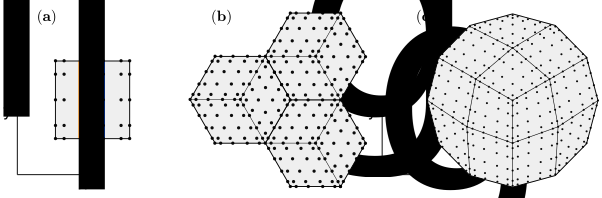
\includegraphics[width=1\linewidth]{Chapter_5/skin_mesh}
	%	\end{center}
	\caption{The mesh with the node distribution, (\textbf{a}) spectral element used for modeling the wall of the core, (\textbf{b}) excerpt of the skin plate and (\textbf{c}) cyanoacrylate glue mesh generated in Gmsh.}
	\label{fig:skin_mesh}
\end{figure}

The \ac{pzt} mesh coincides with the glue mesh.
The convergence of the solution requires time increment to be less than a critical value, above which the displacements go to infinity.
The critical value of time increment depends on the mesh size and the wave mode velocity.
In the present model, convergence was achieved for 3e{$-$9} s.
Additionally, the following number of nodes in the elements were used: the core \(6 \times 5\), epoxy adhesive and cyanoacrylate glue \(6 \times 6\), the plate \(6 \times 6 \times 4\) and \acp{pzt} \(6 \times 6 \times 3\).